%=========================================================
\section{Questões:}

Responda às questões abaixo com base nos conceitos de Movimento Retilíneo Uniforme (MRU) e na análise de seus gráficos.

\begin{enumerate}
    
    \item No gráfico de posição por tempo ($s \times t$) do MRU, a inclinação da reta em relação ao eixo horizontal fornece uma informação física fundamental. Essa inclinação é numericamente igual a:
    \begin{enumerate}[label=(\alph*)]
        \item A aceleração constante do móvel.
        \item A posição inicial ($s_0$) de onde o móvel partiu.
        \item A velocidade escalar média do movimento.
        \item O deslocamento total efetuado pelo corpo.
    \end{enumerate}

    \item Analise a função horária $s = 50 - 2t$ (unidades no SI). Sobre o movimento descrito por essa equação, é correto afirmar que:
    \begin{enumerate}[label=(\alph*)]
        \item O movimento é progressivo, pois a posição inicial é positiva.
        \item O móvel encontra-se em repouso no instante $t = 25$ s.
        \item O movimento é retrógrado, indicando que o móvel caminha contra a orientação da trajetória.
        \item A velocidade do móvel aumenta em 2 m/s a cada segundo que passa.
    \end{enumerate}

    \item Durante a construção de um gráfico $s \times t$, um aluno percebe que a reta cruza o eixo horizontal exatamente no valor $t = 4$ s. O significado físico desse ponto de intersecção é:
    \begin{enumerate}[label=(\alph*)]
        \item O instante em que o móvel inverte o sentido do seu movimento.
        \item O instante em que o móvel passa pela origem das posições ($s = 0$).
        \item O momento em que o cronômetro foi acionado pelo observador.
        \item O ponto de maior velocidade atingida pelo móvel na trajetória.
    \end{enumerate}

    \item Por que é indispensável manter uma escala constante (ex: cada 1 cm na régua valendo sempre 10 m no papel) ao desenhar os eixos de um gráfico de MRU?
    \begin{enumerate}[label=(\alph*)]
        \item Apenas por uma questão de estética e organização visual da apostila.
        \item Para garantir que a reta do gráfico sempre comece na origem (0,0).
        \item Para evitar que a representação visual da velocidade sofra distorções, mantendo a linearidade da reta.
        \item Para que o ângulo de inclinação seja obrigatoriamente de $45^\circ$.
    \end{enumerate}

    \item Se dobrarmos o valor da velocidade de um móvel em MRU, como essa alteração será observada visualmente no gráfico de posição por tempo?
    \begin{enumerate}[label=(\alph*)]
        \item A reta se tornará uma parábola voltada para cima.
        \item A reta ficará mais "em pé" (maior inclinação em relação ao eixo horizontal).
        \item A reta se deslocará verticalmente, alterando o valor de $s_0$.
        \item A reta se tornará perfeitamente horizontal, paralela ao eixo do tempo.
    \end{enumerate}

\end{enumerate}

%=========================================================
\section{Exercícios:}

\begin{enumerate}

    % Exercício 1: Interpretação de Tabela
    \item Um móvel realiza um movimento retilíneo cuja tabela de posições em função do tempo é dada abaixo:
    \begin{center}
        \begin{tabular}{l|ccccc}
            \toprule
            $t$ (s) & 0 & 2 & 4 & 6 & 8 \\ \midrule
            $s$ (m) & 20 & 30 & 40 & 50 & 60 \\ \bottomrule
        \end{tabular}
    \end{center}
    Determine a velocidade escalar do móvel e escreva sua função horária das posições.

    % Exercício 2: Função Horária Simples
    \item Um ponto material movimenta-se sobre uma trajetória retilínea obedecendo à função horária $s = -15 + 3t$ (SI). Determine:
    \begin{enumerate}[label=\alph*)]
        \item A posição inicial e a velocidade.
        \item A posição do móvel no instante $t = 10$ s.
        \item O instante em que o móvel passa pela origem das posições ($s = 0$).
    \end{enumerate}

    % Exercício 3: Distância e Tempo
    \item Um carro mantém uma velocidade constante de \qty{72}{km/h} em uma rodovia retilínea. Calcule a distância percorrida pelo veículo após \qty{15}{minutos} de viagem.

    % Exercício 4: Análise Gráfica (Progressivo/Retrógrado)
    \item Um objeto move-se de acordo com o gráfico $s \times t$ abaixo. Determine a velocidade do objeto e classifique o movimento como progressivo ou retrógrado.
    \cref{fig:exemplo_grafico_2026}
    % (Inserir aqui o código TikZ simplificado da reta descendo de 40 para 0 em 8s)

    \begin{figure}[H]
    \centering
    \begin{tikzpicture}
        \begin{axis}[
            axis lines = left,
            xlabel = {$t$ (s)},
            ylabel = {$s$ (m)},
            % Ajuste para 5 segundos
            xmin=0, xmax=6,
            ymin=0, ymax=50,
            xtick={0, 1, 2, 3, 4, 5},
            ytick={0, 10, 20, 30, 40},
            grid = major,
            grid style = {dashed, gray!30},
            width=0.8\textwidth, height=7cm
        ]

            \addplot [domain=0:5, thick, red] {40 - 8*x} 
                node[pos=0.8, sloped, above] {};

            \draw [dashed, black!60] (axis cs:3.33,0) -- (axis cs:3.33,13.33);
            \draw [dashed, black!60] (axis cs:0,13.33) -- (axis cs:3.33,13.33);
            
        \end{axis}
    \end{tikzpicture}
    \caption{Gráfico que descreve o movimento de um objeto móvel. \label{fig:exemplo_grafico_2026}}
\end{figure}

    % Exercício 5: Conversão de Unidades
    \item A função horária de um projétil é $s = 100 + 20t$ (SI). Qual será a posição deste projétil, em quilômetros, após \qty{2}{minutos} de movimento?

    % Exercício 6: Comparação de Velocidades
    \item Dois móveis, A e B, possuem as seguintes funções horárias: $s_A = 10 + 2t$ e $s_B = 40 - 3t$ (SI). Determine o instante e a posição em que esses dois móveis se encontram.

    % Exercício 7: Velocidade Média em Trechos
    \item Um ciclista percorre \qty{4}{km} com velocidade constante de \qty{12}{km/h} e, em seguida, mais \qty{6}{km} com velocidade constante de \qty{18}{km/h}. Determine o tempo total do percurso.

    % Exercício 8: Gráfico de Velocidade
    \item Desenhe o gráfico de velocidade por tempo ($v \times t$) para um móvel que se desloca segundo a função $s = 50 - 5t$ (SI), para o intervalo de 0 a \qty{10}{s}.

    % Exercício 9: Ultrapassagem
    \item Um trem de \qty{100}{m} de comprimento atravessa uma ponte de \qty{50}{m} com velocidade constante de \qty{15}{m/s}. Quanto tempo o trem leva para atravessar completamente a ponte?

    % Exercício 10: Desafio de Escala
    \item Um aluno deseja construir um gráfico para a função $s = 5 + 25t$. Se ele utilizar uma régua e adotar a escala de \qty{1}{cm} para cada \qty{5}{m} no eixo vertical, a que altura (em cm) estará o ponto correspondente ao instante $t = 3$ s?

\end{enumerate}

%=========================================================
\section{Problemas:}

\begin{enumerate}

    % Problema 1: Encontro de Móveis com Sentidos Opostos
    \item Duas cidades, A e B, estão separadas por uma distância de \qty{300}{km}. No mesmo instante, um carro parte da cidade A em direção a B com velocidade constante de \qty{80}{km/h}, enquanto um caminhão parte de B em direção a A com velocidade constante de \qty{70}{km/h}. 
    \begin{enumerate}[label=\alph*)]
        \item Determine as funções horárias das posições para ambos os veículos, adotando a cidade A como a origem ($s=0$).
        \item Calcule após quanto tempo os veículos se encontrarão na rodovia.
        \item Qual a posição do ponto de encontro em relação à cidade A?
    \end{enumerate}

    % Problema 2: Ultrapassagem e Comprimento
    \item Um trem de carga de \qty{200}{m} de comprimento viaja com velocidade constante de \qty{36}{km/h}. Ele deve atravessar completamente um túnel de \qty{100}{m} de extensão. 
    \begin{enumerate}[label=\alph*)]
        \item Converta a velocidade do trem para metros por segundo (\unit{m/s}).
        \item Qual é a distância total que o trem deve percorrer para que o último vagão saia completamente do túnel?
        \item Quanto tempo, em segundos, dura a travessia completa?
    \end{enumerate}

    % Problema 3: Interpretação de Gráficos de Encontro
    \item Dois móveis, $M_1$ e $M_2$, caminham sobre a mesma trajetória retilínea. O gráfico abaixo representa as suas posições em função do tempo:
    \cref{fig:referencia_grafico_desafio}
    
    \begin{center}
    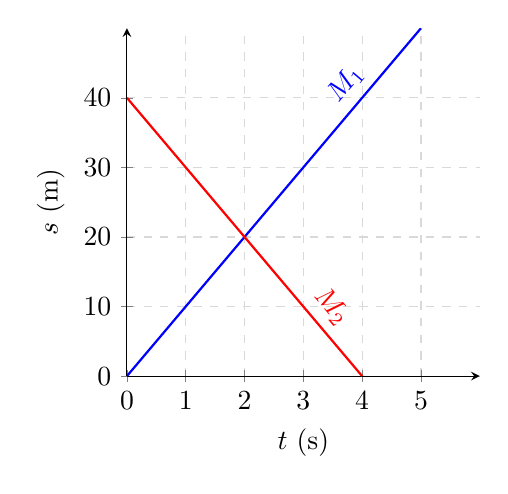
\begin{tikzpicture}
        \begin{axis}[
            axis lines = left,
            xlabel = {$t$ (s)},
            ylabel = {$s$ (m)},
            xmin=0, xmax=6,
            ymin=0, ymax=50,
            xtick={0,1,2,3,4,5},
            ytick={0,10,20,30,40},
            grid = major,
            grid style={dashed, gray!30},
            width=0.5\textwidth, height=6cm
        ]
            % Móvel 1 (Parte do 0 com v=10)
            \addplot [domain=0:5, thick, blue] {10*x} node[pos=0.8, sloped, above] {$M_1$};
            % Móvel 2 (Parte do 40 com v=-10)
            \addplot [domain=0:4, thick, red] {40 - 10*x} node[pos=0.8, sloped, above] {$M_2$};
        \end{axis}
    \end{tikzpicture}
    \label{fig:referencia_grafico_desafio}
    \end{center}
    
    A partir da análise do gráfico, determine:
    \begin{enumerate}[label=\alph*)]
        \item As funções horárias de $M_1$ e $M_2$.
        \item O instante exato em que os móveis se cruzam.
        \item A classificação (progressivo ou retrógrado) de cada movimento.
    \end{enumerate}

\end{enumerate}